% Provenance (never printed): see sources/outline_sources.md (Year 2: interstellar
% medium, molecular clouds, gravitational collapse and the Jeans criterion, protostars
% and protostellar discs). Curves from figdata/bachelor-2/jeans.py; exercise and problem
% values in the Book 4 scratch calculator calc/ch01.py.
\chapter{星际介质与恒星形成}\label{ch:b2:ism-star-formation}

在金牛座方向、距太阳约 \qty{140}{\parsec} 处，
一块暗斑遮住了其后的恒星。用调谐到
一氧化碳谱线的射电望远镜观测，这块暗斑是一团冷气体云，
质量约为太阳的两万倍，其中布满丝状结构；在最致密的团块中，
年轻恒星正在诞生，其中之一 HL 金牛座周围有一个尘埃盘，
盘上呈现明暗相间的环状结构，那里或许已有行星正在形成。
太阳、地球以及本书岩石中的每一个原子，都曾经位于这样的云中。
本章追踪一个行星系统的物质，从恒星之间稀薄的气体，
到新生恒星周围的盘：\omterm{def:b2:ism-star-formation:ism}{星际介质}由什么构成，
为什么依靠自身热能支撑的云最终会坍缩，
坍缩需要多久，恒星如何聚集自身的质量，
以及未能落入恒星的物质为何会形成一个盘。

\begin{recall}
处于主序的恒星在核心通过氢聚变为氦而发光，
并依靠内部压强抵抗自身重量，从而维持自身稳定；
它在赫茨普龙–罗素图中的位置由其质量决定（物理，本科三年级）。
绕质量为 $M$ 的天体做闭合轨道运动的物体，
服从开普勒第三定律 $T^2 = 4\pi^2 a^3/(GM)$（物理，本科一年级）。
温度为 $T$ 的黑体，单位面积发出 $\sigma T^4$ 的辐射（物理，本科二年级）。
在由 $N$ 个粒子组成的理想气体中，
平动的平均动能为 $\tfrac32 N k_{\mathrm B} T$。秒差距
\qty{3.086e16}{m}，是本科一年级分册中的距离单位。
\end{recall}

\section{恒星之间的物质}

恒星之间的空间并非空无一物。在太阳附近，平均
每立方厘米约有一个氢原子，质量密度为
\qty{2.7e-24}{g.cm^{-3}}；我们呼吸的空气中，同样体积内的
分子数约多 $10^{19}$ 倍（见\cref{exo:b2:ism-star-formation:1}）。在整个银河系范围内，这些稀薄物质
仍占银盘质量的
\qtyrange{10}{15}{\percent}。
% ledger: ferriere:mean-density, ferriere:disc-fraction

\begin{definition}[星际介质，星际尘埃]
\label{def:b2:ism-star-formation:ism}
\emph{星际介质}\index{星际介质}是充满
星系中恒星之间空间的气体和尘埃。\emph{星际尘埃}\index{星际尘埃}是其中以
固态颗粒存在的部分，颗粒直径从几纳米
到约一微米，由硅酸盐、碳化合物
以及在低温区域中的冰构成。
\end{definition}

其组成与在太阳和陨石中测得的一致：按质量计，
氢占 \qty{70.4}{\percent}，氦占 \qty{28.1}{\percent}，
较重元素占 \qty{1.5}{\percent}。尘埃的质量仅占 \qtyrange{0.5}{1}{\percent}，
但某些元素的大部分都在尘埃中：气体中镁、硅和铁的含量
比太阳低 10 至 100 倍，原因是这些原子被锁定在颗粒之中；
而碳、氮和氧的亏损仅为 1.2 至 3 倍。这些颗粒是未来行星系统
最初的固体，
在\cref{ch:b2:planet-formation-meteorites}中
将追踪它们。
% ledger: ferriere:composition, ferriere:dust-fraction, ferriere:refractory-depletion

\subsection{五种相}

气体远非均匀。它呈现出几种不同的状态，即相，
每种相都有其特定的温度和密度范围（见下表）。约一半的质量
处于仅占 \qtyrange{1}{2}{\percent} 体积的云中；
其余的温热或高温气体则充满云之间的空间。
% ledger: ferriere:disc-fraction

\begin{table}[htbp]
\centering
\small
\begin{tabular}{lll}
\hline
相 & 温度 (K) & 数密度 $n$ (\unit{cm^{-3}}) \\
\hline
\omterm{def:b2:ism-star-formation:molecular-cloud}{分子云} & 10--20 & $10^2$--$10^6$ \\
冷原子气体 & 50--100 & 20--50 \\
温原子气体 & 6000--10\,000 & 0.2--0.5 \\
温电离气体 & 约 8000 & 0.2--0.5 \\
高温电离气体 & 约 $10^6$ & 约 0.0065 \\
\hline
\end{tabular}
\caption{太阳附近星际气体的各种相；$n$ 为
氢核的数密度。}
\label{tab:b2:ism-star-formation:phases}
% ledger: ferriere:molecular, ferriere:cold-atomic, ferriere:warm-atomic, ferriere:warm-ionized, ferriere:hot-ionized
\end{table}

该表中隐含着一个规律。理想气体的压强为
$P = n k_{\mathrm B} T$，因此乘积 $nT$ 可以度量压强。对于冷原子气体，
$nT$ 约为 $30\times75 \approx 2000$（单位为 \unit{K.cm^{-3}}）；对于温原子气体，
约为 $0.3\times8000 \approx 2400$；对于高温气体，约为
$0.0065\times10^6 = 6500$。在相差不超过几倍的范围内，占据云间空间的三种相
处于相同的压强下（见下图）。
当热气体与冷气体在相等压强下接触时，二者都不会将对方推开；
一块在恒压下冷却的气体，密度按比例增大，
并从温相转入冷相。\omterm{def:b2:ism-star-formation:molecular-cloud}{分子云}的压强要高得多，在其致密部分可高出数千倍：
它们靠自身引力束缚在一起，而不是靠周围环境的压强。

\begin{omfigure}
\begin{tikzpicture}
\begin{axis}[omrecord, width=0.86\linewidth, height=6.4cm, xmode=log, ymode=log,
  xmin=1e-3, xmax=1e7, ymin=3, ymax=3e6,
  xlabel={氢核数密度 $n$ (\unit{cm^{-3}})}, ylabel={温度 $T$ (K)},
  tick label style={font=\scriptsize}, label style={font=\small}, clip=false,
  legend pos=north east, legend style={font=\scriptsize, draw=black!30}]
\addplot[black!45, densely dashed, domain=1e-3:1e3, samples=2] {3000/x};
\addlegendentry{$nT = \num{3000}$}
\addplot[black!60, densely dotted, thick, domain=0.1:1e5, samples=2] {3e5/x};
\addlegendentry{$nT = 3\times10^5$}
\fill[blue!45, opacity=0.6] (axis cs:1e2,10) rectangle (axis cs:1e6,20);
\fill[teal!50, opacity=0.6] (axis cs:20,50) rectangle (axis cs:50,100);
\fill[orange!55, opacity=0.6] (axis cs:0.2,6000) rectangle (axis cs:0.5,10000);
\fill[red!45, opacity=0.6] (axis cs:0.2,5714) rectangle (axis cs:0.5,11200);
\fill[violet!50, opacity=0.6] (axis cs:0.00464,7.14e5) rectangle (axis cs:0.0091,1.4e6);
\node[font=\scriptsize, anchor=south east] at (axis cs:1e6,20) {分子云};
\node[font=\scriptsize, anchor=south west] at (axis cs:50,100) {冷原子气体};
\node[font=\scriptsize, anchor=east, align=right] at (axis cs:0.17,8000) {温原子气体 \\与温电离气体};
\node[font=\scriptsize, anchor=west] at (axis cs:0.011,1e6) {高温电离气体};
\end{axis}
\end{tikzpicture}

\par\smallskip{\small 太阳附近星际气体的各相（上表所列范围；
温电离相与高温相以单一数值给出，画成宽为 1.4 倍的方框）。
沿每条灰线，压强 $nk_{\mathrm B}T$ 为常数：
冷相、温相与热相的压强彼此接近，相差在几倍之内，
而\omterm{def:b2:ism-star-formation:molecular-cloud}{分子云}依靠自身引力束缚，压强可高出数千倍。
数据来源：Ferrière（2001）。}
\end{omfigure}

尘埃以三种方式显示自身。它使其后方恒星的光变暗，
并且对蓝光的减弱比对红光更强，因此透过尘埃所见的恒星
比实际更红。它在远红外和毫米波段发光，
其温度约为几十开尔文，即星光加热它所达到的温度。此外，
它还会把致密云团内部的东西挡在光学望远镜之外，
因此恒星形成要在射电与红外波段观测。气体则通过其谱线被追踪：
原子氢通过 \qty{21}{cm} 的射电谱线，
分子氢在低温时几乎不辐射，因此通过与之伴随的分子的谱线追踪，
其中首推一氧化碳。

\section{分子云}

最冷、最致密的相是恒星形成之处。

\begin{definition}[分子云，致密云核]
\label{def:b2:ism-star-formation:molecular-cloud}
称\emph{分子云}\index{分子云}为\omterm{def:b2:ism-star-formation:ism}{星际介质}中的一个区域，
其密度足够高、足够不透明，使氢大部分以分子形式存在，
即 \ce{H2}，并受尘埃屏蔽，免受会将其打散的恒星紫外线照射；
其温度约为 \qty{10}{K} 至 \qty{20}{K}。
一个\emph{致密云核}\index{致密云核}是分子云内部的紧凑凝聚体，
尺度为几十分之一秒差距或更小，密度为
每立方厘米 $10^4$ 至 $10^5$ 个粒子，由此
形成单颗恒星或一小群恒星。
\end{definition}

云团按层级组织（见下表）。像金牛座这样的暗云
包含云块，云块包含云核，每一级都比上一级更致密、更小、也更安静：
在云核中，气体运动速度至多只有零点几千米每秒，
相当于 \qty{10}{K} 时气体中的声速。金牛座中以一氧化碳成图的
区域约含 \num{2.4e4} 个太阳质量的
气体；其中只有 \qtyrange{0.3}{1.2}{\percent} 转化为
那里所见的年轻恒星，形成速率约为每十万年八颗恒星，
在过去三百万年间如此。恒星形成既缓慢又浪费。
% ledger: bt07:clouds, bt07:clumps, bt07:cores, goldsmith:taurus-mass, goldsmith:taurus-sfe, goldsmith:taurus-distance

\begin{table}[htbp]
\centering
\small
\begin{tabular}{lccc}
\hline
 & 暗云 & 云块 & \omterm{def:b2:ism-star-formation:molecular-cloud}{致密云核} \\
\hline
质量（太阳质量） & $10^3$--$10^4$ & 50--500 & 0.5--5 \\
线度（pc） & 2--15 & 0.3--3 & 0.03--0.2 \\
平均密度（\unit{cm^{-3}}） & 50--500 & $10^3$--$10^4$ & $10^4$--$10^5$ \\
气体温度（K） & 约 10 & 10--20 & 8--12 \\
实例 & 金牛座、苍蝇座 &——& L1544, B68 \\
\hline
\end{tabular}
\caption{暗\omterm{def:b2:ism-star-formation:molecular-cloud}{分子云}的层级结构。密度计入
所有粒子。数据来源：Bergin 和 Tafalla（2007）。}
\label{tab:b2:ism-star-formation:hierarchy}
% ledger: bt07:clouds, bt07:clumps, bt07:cores
\end{table}

为什么云团如此寒冷？气体通过发射能够逃逸的光子而失去能量，
而分子是高效的发射体：一次碰撞使一氧化碳
分子跃迁到较高的转动能级，分子随后
通过发射毫米波段的光子回落，光子离开云团，
并带走碰撞的能量。尘埃被透入的微弱星光加热，
并在远红外波段辐射。加热源包括宇宙线，
以及经尘埃滤过的星光，其作用很弱；平衡
最终稳定在 \qty{10}{K} 附近。在这样的气体中，热压很小，引力可以
占上风。

\begin{omfigure}
\begin{minipage}[c]{0.44\linewidth}
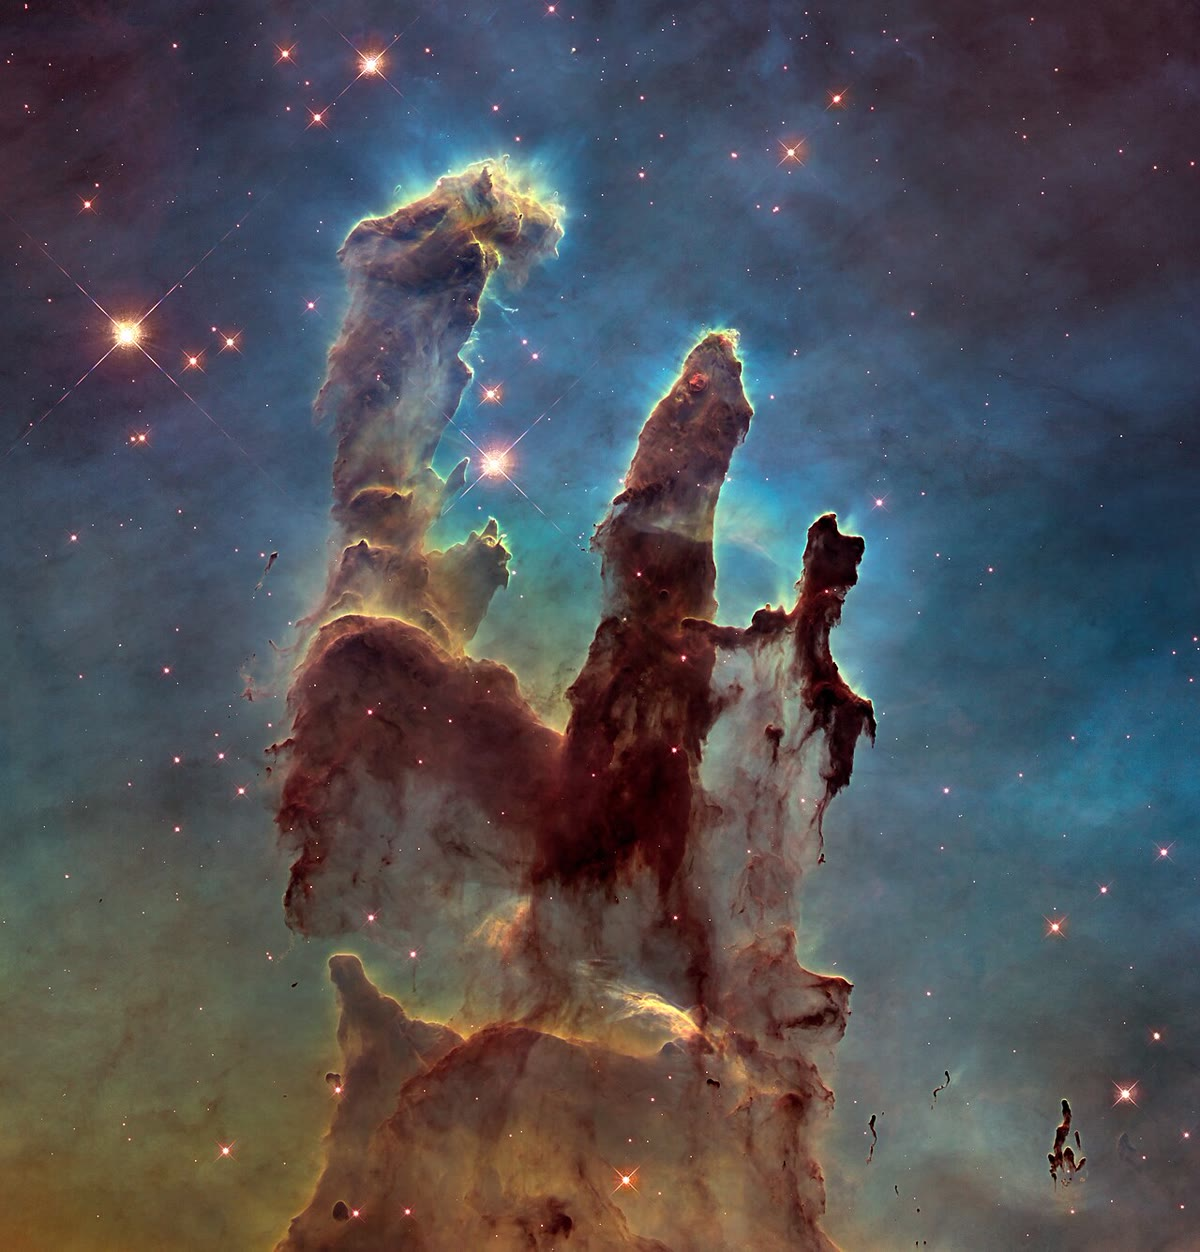
\includegraphics[width=\linewidth]{images/book4/b2-pillars-of-creation.jpg}
\end{minipage}\hfill
\begin{minipage}[c]{0.52\linewidth}
{\small 鹰状星云中的“创生之柱”，由哈勃
空间望远镜以可见光成像。这些柱状结构是冷的致密分子气体与
尘埃，长达数光年，被画面外大质量年轻恒星的紫外线从上方照亮并受侵蚀；
尘埃使其不透明。
顶端的小凝聚体正在形成恒星。NASA、ESA 与哈勃
Heritage Team（STScI/AURA），公有领域。}
\end{minipage}
\end{omfigure}

\section{引力坍缩}

云团是两种能量之间的平衡：其气体的热能，
向外推，而其引力势能向内拉。
后者随质量增长得比前者更快；超过某一质量后，引力
便占上风。

\begin{proposition}[均匀球体的引力势能]
\label{prop:b2:ism-star-formation:grav-energy}
设密度均匀、质量为 $M$、半径为 $R$ 的球体，
其引力势能为
\[
  U = -\frac{3}{5}\,\frac{G M^2}{R}.
\]
\end{proposition}

\begin{proof}
将球体逐壳层构造。当半径为 $r$ 时，它的质量为
$m(r) = M r^3/R^3$；将厚度为 $\mathrm dr$、质量为
$\mathrm dm = 3M r^2\,\mathrm dr/R^3$ 的壳层从无穷远移到其表面时，释放
能量 $G m(r)\,\mathrm dm/r$，因为球体在其外部的吸引力，等同于
其质量集中于球心时的吸引力（壳层定理，物理学中的结论）。由此
\[
  U = -\int_0^R \frac{G}{r}\,\frac{M r^3}{R^3}\,\frac{3 M r^2}{R^3}\,\mathrm dr
    = -\frac{3 G M^2}{R^6}\int_0^R r^4\,\mathrm dr = -\frac{3}{5}\,\frac{G M^2}{R}.
  \qedhere
\]
\end{proof}

处于平衡态的自引力天体满足位力定理：对时间取平均后，
其动能的两倍与引力能之和为零，
$2K + U = 0$（物理学，本科三年级，
由运动方程推出）。对于静止的云团，$K$ 为其粒子的
热能。若 $2K > |U|$，气体膨胀；若 $2K < |U|$，
则引力无平衡态与之抗衡，云团收缩。

\begin{proposition}[金斯判据]\label{prop:b2:ism-star-formation:jeans}
温度为 $T$、密度为 $\rho$ 的均匀等温云团，
由平均质量为 $\mu m_u$ 的粒子组成，在自身引力作用下垮塌，
若其质量超过\emph{\omterm{def:b2:ism-star-formation:jeans}{金斯质量}}：
\[
  M_J = \left(\frac{5 k_{\mathrm B} T}{G\mu m_u}\right)^{3/2}
        \left(\frac{3}{4\pi\rho}\right)^{1/2},
\]
或等价地，若其半径超过\emph{\omterm{def:b2:ism-star-formation:jeans}{金斯长度}}：
\[
  R_J = \left(\frac{15 k_{\mathrm B} T}{4\pi G\mu m_u\,\rho}\right)^{1/2}.
\]
这就是\emph{金斯判据}\index{金斯判据}。
\end{proposition}

\begin{proof}
云团含有 $N = M/(\mu m_u)$ 个粒子，其热能为
$K = \tfrac32 N k_{\mathrm B}T = \tfrac32 M k_{\mathrm B}T/(\mu m_u)$。由
\cref{prop:b2:ism-star-formation:grav-energy}可知，若
$2K < \tfrac35 GM^2/R$，即
\[
  \frac{3 M k_{\mathrm B} T}{\mu m_u} < \frac{3}{5}\,\frac{G M^2}{R}
  \iff M > \frac{5 k_{\mathrm B} T}{G \mu m_u}\, R .
\]
消去 $R$，利用 $M = \tfrac43\pi R^3\rho$，即 $R = (3M/4\pi\rho)^{1/3}$：
$M^{2/3} > \frac{5 k_{\mathrm B}T}{G\mu m_u}\,(3/4\pi\rho)^{1/3}$，两边同时
取 $3/2$ 次幂，得 $M > M_J$。若改为消去 $M$，
$\tfrac43\pi R^3\rho > 5 k_{\mathrm B}T R/(G\mu m_u)$，得 $R^2 > 15
k_{\mathrm B}T/(4\pi G\mu m_u\rho)$，即 $R > R_J$。
\end{proof}

\begin{definition}[金斯质量、金斯长度]\label{def:b2:ism-star-formation:jeans}
\emph{金斯质量}\index{金斯质量} $M_J$ 与
\emph{金斯长度}\index{金斯长度} $R_J$ 分别是给定温度和密度的气体的
临界质量与临界半径：超过该值时，由此气体构成的均匀球体
在自身引力作用下垮塌（见\cref{prop:b2:ism-star-formation:jeans}）。
\end{definition}

\omterm{def:b2:ism-star-formation:jeans}{金斯质量}随 $T^{3/2}$ 增大，随 $\rho^{-1/2}$ 减小：冷而致密的气体
最容易垮塌。在\omterm{def:b2:ism-star-formation:molecular-cloud}{分子云}中，粒子的平均质量为
$\mu = 2.33$ 个原子质量单位，成分为分子氢，
并约每五个分子含一个氦原子。在 \qty{10}{K}、每立方厘米 $10^4$ 个粒子的条件下，
$\rho = \mu m_u n = \qty{3.87e-17}{kg.m^{-3}}$，且
$M_J = 5.5$ 个太阳质量，对应\omterm{def:b2:ism-star-formation:jeans}{金斯长度}为 \qty{0.13}{\parsec}：
这即\omterm{def:b2:ism-star-formation:molecular-cloud}{致密云核}的质量与尺度。在暗云的平均密度下，
每立方厘米 $100$ 个粒子，\omterm{def:b2:ism-star-formation:jeans}{金斯质量}大十倍，为 55
个太阳质量；质量为 \num{24000} 个太阳质量的云团，如金牛座\omterm{def:b2:ism-star-formation:molecular-cloud}{分子云}，含有
数百个这样的云核（见下图）。
% ledger: kauffmann:mu, nist:u, const:kB, const:G, sun:mass, goldsmith:taurus-mass

\begin{omfigure}
\begin{tabular}{@{}c@{\hspace{3mm}}c@{}}
\begin{tikzpicture}
\begin{axis}[omrecord, width=0.455\linewidth, height=6.0cm, xmode=log, ymode=log,
  xmin=10, xmax=1e7, ymin=0.05, ymax=1e4,
  xlabel={$n$ (\unit{cm^{-3}})}, ylabel={金斯质量（太阳质量）},
  tick label style={font=\scriptsize}, label style={font=\small},
  legend style={font=\scriptsize, at={(0.97,0.97)}, anchor=north east, draw=none, fill=white, fill opacity=0.85}]
\fill[blue!12] (axis cs:1e4,0.5) rectangle (axis cs:1e5,5);
\node[font=\scriptsize, blue!50!black, anchor=north east] at (axis cs:1e5,0.5) {致密云核};
\addplot[very thick, blue!70!black] table[x=n, y=MJ10] {figdata/out/bachelor-2-jeans-jeans.dat};
\addlegendentry{\qty{10}{K}}
\addplot[very thick, orange!80!black] table[x=n, y=MJ20] {figdata/out/bachelor-2-jeans-jeans.dat};
\addlegendentry{\qty{20}{K}}
\addplot[very thick, red!75!black] table[x=n, y=MJ50] {figdata/out/bachelor-2-jeans-jeans.dat};
\addlegendentry{\qty{50}{K}}
\end{axis}
\end{tikzpicture}
&
\begin{tikzpicture}
\begin{axis}[omrecord, width=0.455\linewidth, height=6.0cm, xmode=log, ymode=log,
  xmin=10, xmax=1e7, ymin=0.01, ymax=20,
  xlabel={$n$ (\unit{cm^{-3}})}, ylabel={自由落体时标（Ma）},
  tick label style={font=\scriptsize}, label style={font=\small}]
\addplot[very thick, black!70] table[x=n, y=tff_Myr] {figdata/out/bachelor-2-jeans-tff.dat};
\fill[blue!12] (axis cs:1e4,0.05) rectangle (axis cs:1e5,0.5);
\addplot[very thick, black!70] table[x=n, y=tff_Myr] {figdata/out/bachelor-2-jeans-tff.dat};
\node[font=\scriptsize, blue!50!black, anchor=north] at (axis cs:3.2e4,0.05) {致密云核};
\end{axis}
\end{tikzpicture}
\\[2pt]
{\small (a) \omterm{def:b2:ism-star-formation:jeans}{金斯质量}} & {\small (b) \omterm{def:b2:ism-star-formation:free-fall}{自由落体时标}}
\end{tabular}

\par\smallskip{\small (a) 三种温度下\omterm{def:b2:ism-star-formation:jeans}{金斯质量}随数密度的变化
（$\mu = 2.33$）。阴影框标出观测到的\omterm{def:b2:ism-star-formation:molecular-cloud}{致密云核}的质量与密度：
在 \qty{10}{K} 下，它们的质量接近\omterm{def:b2:ism-star-formation:jeans}{金斯质量}。（b）
\omterm{def:b2:ism-star-formation:free-fall}{自由落体时标}（见\cref{prop:b2:ism-star-formation:free-fall}）：
每立方厘米 $10^4$ 个粒子时约为三十三万年，在每立方厘米 $10^2$ 个粒子时则长十倍。}
\end{omfigure}

开始垮塌的云团密度增大，其\omterm{def:b2:ism-star-formation:jeans}{金斯质量}随
$\rho^{-1/2}$ 减小，只要它能辐射出
压缩产生的热量，它就保持低温。随后，云团的碎块各自失稳，
并独立垮塌：云团发生\emph{碎裂}。这既解释了恒星为何成群形成，
也解释了恒星质量为何远小于形成它们的云团。
当气体致密到辐射无法逸出时，碎裂停止：
压缩热被截留，温度升高，
\omterm{def:b2:ism-star-formation:jeans}{金斯质量}不再减小。

垮塌需要多长时间？若压强可忽略不计，云团的每一壳层
都将自由下落，朝中心运动。

\begin{proposition}[自由落体时标]\label{prop:b2:ism-star-formation:free-fall}
密度为 $\rho$ 的均匀球体，初始静止且无压强，
垮塌至其中心所需的时间为
\[
  t_{\mathrm{ff}} = \left(\frac{3\pi}{32\,G\rho}\right)^{1/2},
\]
与其半径无关。
\end{proposition}

\begin{proof}
考虑位于球面上、距中心距离为 $R$ 的一个静止质点。
其内部的壳层下落得更快或与之同步，
决不落后，因此吸引它的质量 $M = \tfrac43\pi R^3\rho$ 始终保持不变。
其轨迹是一个退化的开普勒轨道，即被压扁为直线段的椭圆，
远端位于 $R$ 处，吸引中心位于
另一端，因此其半长轴为 $a = R/2$。从远端
落到中心需要半个周期；由开普勒第三定律
\[
  t_{\mathrm{ff}} = \frac12\cdot 2\pi\sqrt{\frac{(R/2)^3}{GM}}
  = \pi\sqrt{\frac{R^3}{8\,G\cdot\frac43\pi R^3\rho}}
  = \sqrt{\frac{3\pi}{32\,G\rho}} .
\]
$R$ 消去：均匀球体的每一壳层都在
同一时刻到达中心。
\end{proof}

\begin{definition}[自由落体时标]\label{def:b2:ism-star-formation:free-fall}
称密度为 $\rho$ 的气体的\emph{自由落体时标}\index{自由落体时标}为
$t_{\mathrm{ff}} = (3\pi/32G\rho)^{1/2}$，即
同一密度的均匀球体仅靠自身引力垮塌所需的时间。
\end{definition}

对于每立方厘米含 $10^4$ 个粒子的\omterm{def:b2:ism-star-formation:molecular-cloud}{致密云核}，其\omterm{def:b2:ism-star-formation:free-fall}{自由落体时标}
为 \qty{0.34}{Ma}；对于数密度为 $10^2$ 的整个暗云，为 \qty{3.4}{Ma}。若银河系的每一个
\omterm{def:b2:ism-star-formation:molecular-cloud}{分子云}都在一个\omterm{def:b2:ism-star-formation:free-fall}{自由落体时标}内垮塌并转化为
恒星，则银河系恒星形成的速度将远快于实际：以金牛座为例，
过去三百万年间真正转化为恒星的气体约占云团的百分之一。
这些云团受湍流运动以及被气体中电离部分拖动的磁场阻滞，
并且其中大部分气体在垮塌前即被最早形成的大质量恒星的风和光驱散，
因此
在金牛座测得的效率很低。
% ledger: bt07:tff

\begin{history}[詹姆斯·金斯]
詹姆斯·金斯（1877--1946）于 1902 年发表了关于气体在
自身引力作用下稳定性的分析，\omterm{def:b2:ism-star-formation:jeans}{金斯质量}和\omterm{def:b2:ism-star-formation:jeans}{金斯长度}即由此导出。他
研究了无限均匀气体中微小密度波的增长，
并发现长于临界长度的波不受压强的抑制，
而是会增长：气体会分裂为约此尺度的凝聚体。他的临界
长度与上文求得的半径仅相差一个数值因子；
两者的物理图像（引力与热压强之间的对抗）是相同的。
\end{history}

\section{原恒星}

\omterm{def:b2:ism-star-formation:molecular-cloud}{致密云核}的垮塌并不均匀。中心略为致密，因而率先
下落；那里形成一个小而致密、温度很高的天体，它靠
吞食不断落到其上的气体而长大。

\begin{definition}[原恒星]\label{def:b2:ism-star-formation:protostar}
称\emph{原恒星}\index{原恒星}为仍处于形成过程中的恒星，其质量
主要通过吸积母云核中的气体而增加；它
依靠下落气体释放的能量发光，而非核聚变。
\end{definition}

\omterm{def:b2:ism-star-formation:protostar}{原恒星}的增长速度有多快？临近垮塌的云核质量约为一个\omterm{def:b2:ism-star-formation:jeans}{金斯质量}，
其垮塌约需一个\omterm{def:b2:ism-star-formation:free-fall}{自由落体时标}，因此质量流入的速率量级为
$M_J/t_{\mathrm{ff}}$。

\begin{proposition}[原恒星的吸积率]
\label{prop:b2:ism-star-formation:accretion}
设 $c_s = (k_{\mathrm B}T/\mu m_u)^{1/2}$ 为
云核气体的等温声速。\omterm{def:b2:ism-star-formation:jeans}{金斯质量}与\omterm{def:b2:ism-star-formation:free-fall}{自由落体时标}之比
与密度无关，并且
\[
  \frac{M_J}{t_{\mathrm{ff}}} \approx 10\,\frac{c_s^3}{G}:
\]
即\omterm{def:b2:ism-star-formation:protostar}{原恒星}的增长速率量级为 $c_s^3/G$，
仅由其云核的温度决定。
\end{proposition}

\begin{proof}
利用 $k_{\mathrm B}T/(\mu m_u) = c_s^2$，$M_J = 5^{3/2}\,c_s^3\,G^{-3/2}
(3/4\pi\rho)^{1/2}$ 和 $t_{\mathrm{ff}} = (3\pi/32)^{1/2}(G\rho)^{-1/2}$，于是
\[
  \frac{M_J}{t_{\mathrm{ff}}} = 5^{3/2}\left(\frac{3}{4\pi}\right)^{1/2}
  \left(\frac{32}{3\pi}\right)^{1/2}\frac{c_s^3}{G}
  = 11.18\times0.489\times1.84\,\frac{c_s^3}{G} \approx 10\,\frac{c_s^3}{G},
\]
其中 $\rho$ 消去。该因子取决于云核的形状；
若模型中云核密度向外递减（与观测相符），则给出的速率
更接近 $c_s^3/G$ 本身。
\end{proof}

在 \qty{10}{K} 时，$c_s = \qty{0.19}{km.s^{-1}}$，$c_s^3/G$ 为
\num{1.6e-6} 太阳质量每年；像太阳这样的恒星约需
\num{600000} 年，这一时间与其云核的\omterm{def:b2:ism-star-formation:free-fall}{自由落体时标}相当。
在温度较高的云核中，\qty{20}{K} 时速率为原来的 $2^{3/2} = 2.8$ 倍。

\begin{omfigure}
\begin{tikzpicture}[font=\scriptsize]
% panel 1: core
\begin{scope}
\shade[inner color=gray!70, outer color=gray!10] (0,0) circle (1.0);
\node[align=center] at (0,-1.45) {(1) 致密云核 \\$\sim\qty{0.1}{pc}$, \qty{10}{K}};
\end{scope}
% panel 2: collapse with infall arrows
\begin{scope}[xshift=3.0cm]
\shade[inner color=gray!80, outer color=gray!10] (0,0) circle (0.9);
\foreach \a in {0,45,...,315} \draw[-{Stealth[length=1.6mm]}, black!70] (\a:0.85) -- (\a:0.3);
\fill[orange!90!red] (0,0) circle (0.07);
\node[align=center] at (0,-1.45) {(2) 垮塌 \\$t_{\mathrm{ff}} \sim \qty{0.1}{Ma}$};
\end{scope}
% panel 3: protostar with disc and outflow
\begin{scope}[xshift=6.0cm]
\fill[gray!25] (0,0) ellipse (0.9 and 0.6);
\fill[brown!55] (0,0) ellipse (0.75 and 0.12);
\fill[orange!90!red] (0,0) circle (0.08);
\fill[blue!25] (0,0.1) -- (-0.22,0.95) -- (0.22,0.95) -- cycle;
\fill[blue!25] (0,-0.1) -- (-0.22,-0.95) -- (0.22,-0.95) -- cycle;
\node[align=center] at (0,-1.45) {(3) 原恒星、原恒星盘 \\和外流，$\sim\qty{0.5}{Ma}$};
\end{scope}
% panel 4: T Tauri with disc
\begin{scope}[xshift=9.0cm]
\fill[brown!55] (0,0) ellipse (0.85 and 0.1);
\fill[yellow!80!orange] (0,0) circle (0.1);
\draw[blue!40, thick] (0,0.15) -- (0,0.6); \draw[blue!40, thick] (0,-0.15) -- (0,-0.6);
\node[align=center] at (0,-1.45) {(4) 金牛 T 型星 \\与原行星盘，1--\qty{5}{Ma}};
\end{scope}
% panel 5: planetary system
\begin{scope}[xshift=12.0cm]
\fill[yellow!80!orange] (0,0) circle (0.12);
\foreach \r in {0.3,0.5,0.8} \draw[black!40] (0,0) ellipse ({\r} and {0.4*\r});
\fill (0.3,0) circle (0.03); \fill (-0.5,0.03) circle (0.035); \fill (0.8,0.05) circle (0.06);
\node[align=center] at (0,-1.45) {(5) 主序星 \\与行星};
\end{scope}
\foreach \x in {1.4,4.4,7.4,10.4} \draw[-{Stealth}, thick, black!60] (\x,0) -- (\x+0.25,0);
\end{tikzpicture}

\par\smallskip{\small 从\omterm{def:b2:ism-star-formation:molecular-cloud}{致密云核}到行星系统（示意图，未按比例绘制）。
(1) 接近\omterm{def:b2:ism-star-formation:jeans}{金斯质量}的冷云核。(2) 其中心首先收缩，
形成\omterm{def:b2:ism-star-formation:protostar}{原恒星}。(3) \omterm{def:b2:ism-star-formation:protostar}{原恒星}通过盘吸积物质而增长，同时\omterm{def:b2:ism-star-formation:t-tauri}{双极外流}
沿自转轴清除气体。(4) 包层耗尽后，\omterm{def:b2:ism-star-formation:t-tauri}{金牛 T 型星}仍
在收缩，并被其盘所环绕。(5) 盘已消散，其中剩余的
固体即为行星。图中时间取自正文的自由落体与吸积估计，
以及上一节的盘寿命。}
\end{omfigure}

\omterm{def:b2:ism-star-formation:protostar}{原恒星}在吸积的同时，依靠落入气体的能量发光。
包层耗尽之后，它仍然发光，但此时并不依靠聚变，
而是依靠收缩。

\begin{proposition}[收缩为年轻恒星提供能量]
\label{prop:b2:ism-star-formation:contraction}
处于平衡态、缓慢收缩的自引力气体球，
会辐射掉所释放的引力能中的一半，另一半保留为热能：
它在失去能量的同时温度升高。
\end{proposition}

\begin{proof}
平衡时由位力定理得 $2K + U = 0$，故总能量
为 $E = K + U = U/2$。若半径缩小，$U$ 减小某个量
$\Delta < 0$；于是 $E$ 改变 $\Delta/2$，这即为辐射出去的
能量，而 $K = -U/2$ 改变 $-\Delta/2 > 0$：热能，进而
温度升高了另一半。
\end{proof}

\begin{definition}[开尔文–亥姆霍兹时标]\label{def:b2:ism-star-formation:kh-time}
称\emph{开尔文–亥姆霍兹时标}\index{开尔文–亥姆霍兹时标}
为质量为 $M$、半径为 $R$、光度为 $L$ 的恒星的
$t_{\mathrm{KH}} = GM^2/(RL)$，它是仅靠收缩即可维持其光度之
时间的数量级。
\end{definition}

对于现在的太阳，$t_{\mathrm{KH}} = \qty{31}{Ma}$：远短于其年龄，
这正是太阳必须燃烧氢的原因。对于质量为一个太阳质量的年轻恒星，
半径和光度均为太阳的两倍，其值为 \qty{8}{Ma}
（见\cref{exo:b2:ism-star-formation:6}）。当中心温度高到足以使氢聚变
来维持光度时，收缩即告结束：恒星到达主序（回顾）。
% ledger: sun:mass, sun:R, sun:L, const:G

\begin{definition}[金牛 T 型星、双极外流]\label{def:b2:ism-star-formation:t-tauri}
\emph{金牛 T 型星}\index{金牛 T 型星}是质量小于约两个太阳质量的年轻恒星，
它已抛去包层而变得可见，但尚未到达主序：
它靠收缩发光，亮度会发生变化，
通常周围环绕着一个仍在向其吸积物质的盘。
\emph{双极外流}\index{双极外流}是年轻恒星
沿其盘的自转轴，向相反方向抛射出的一对快速
气体喷流或风。
\end{definition}

外流带走了盘向恒星输送的气体中的一部分角动量，
并沿轴线清除包层。HL 金牛座的恒星在\omterm{def:b2:ism-star-formation:protostar}{原恒星}阶段末期，
驱动着一股高度准直的
外流。
% ledger: alma:hltau

\section{盘}

\omterm{def:b2:ism-star-formation:molecular-cloud}{致密云核}会缓慢转动：跨越云核时，气体速度梯度
约为每秒差距数个十分之一千米每秒。云核坍缩时，其
角动量守恒，缓慢的自转随之变快。

\begin{proposition}[离心半径]\label{prop:b2:ism-star-formation:centrifugal}
比角动量为 $j$（即单位质量的角动量）的气体，
向质量为 $M$ 的天体下落时无法到达中心：它会落在
一条圆轨道上，其半径为
\[
  r_c = \frac{j^2}{G M}.
\]
\end{proposition}

\begin{proof}
无摩擦时，下落气体的角动量守恒，
因此在距离 $r$ 处其转动速度为 $v = j/r$。若气体能在 $r$ 处绕行，
则引力须恰好提供所需的向心加速度，
即 $GM/r^2 = v^2/r = j^2/r^3$，亦即 $r = j^2/(GM)$。更靠近中心时，
所需的向心加速度 $j^2/r^3$ 超过了引力的拉力，
气体便无法再向内。
\end{proof}

沿自转轴下落的气体角动量很小，
会直接落到恒星上；在赤道面内下落的气体则保持
其转动。从相对两侧、沿不同路径下落的气体，会在
赤道面上下方相互碰撞，失去竖直方向的运动，
并聚集成一个半径约为 $r_c$ 的薄旋转盘。对于一个
\qty{0.1}{pc} 的云核，它约两千万年转动一周，$r_c$ 约为几百
个天文单位（见\cref{exo:b2:ism-star-formation:11}）：与观测到的盘的尺度相当。

\begin{definition}[原行星盘]\label{def:b2:ism-star-formation:disc}
\emph{原行星盘}\index{原行星盘}（或
\emph{原恒星盘}\index{原恒星盘}）是
围绕年轻恒星、近似开普勒转动的扁平气体与尘埃盘，由其母云核中
角动量过大而无法落到恒星上的物质组成；
行星正是在其中形成的。
\end{definition}

\begin{omfigure}
\begin{minipage}[c]{0.44\linewidth}
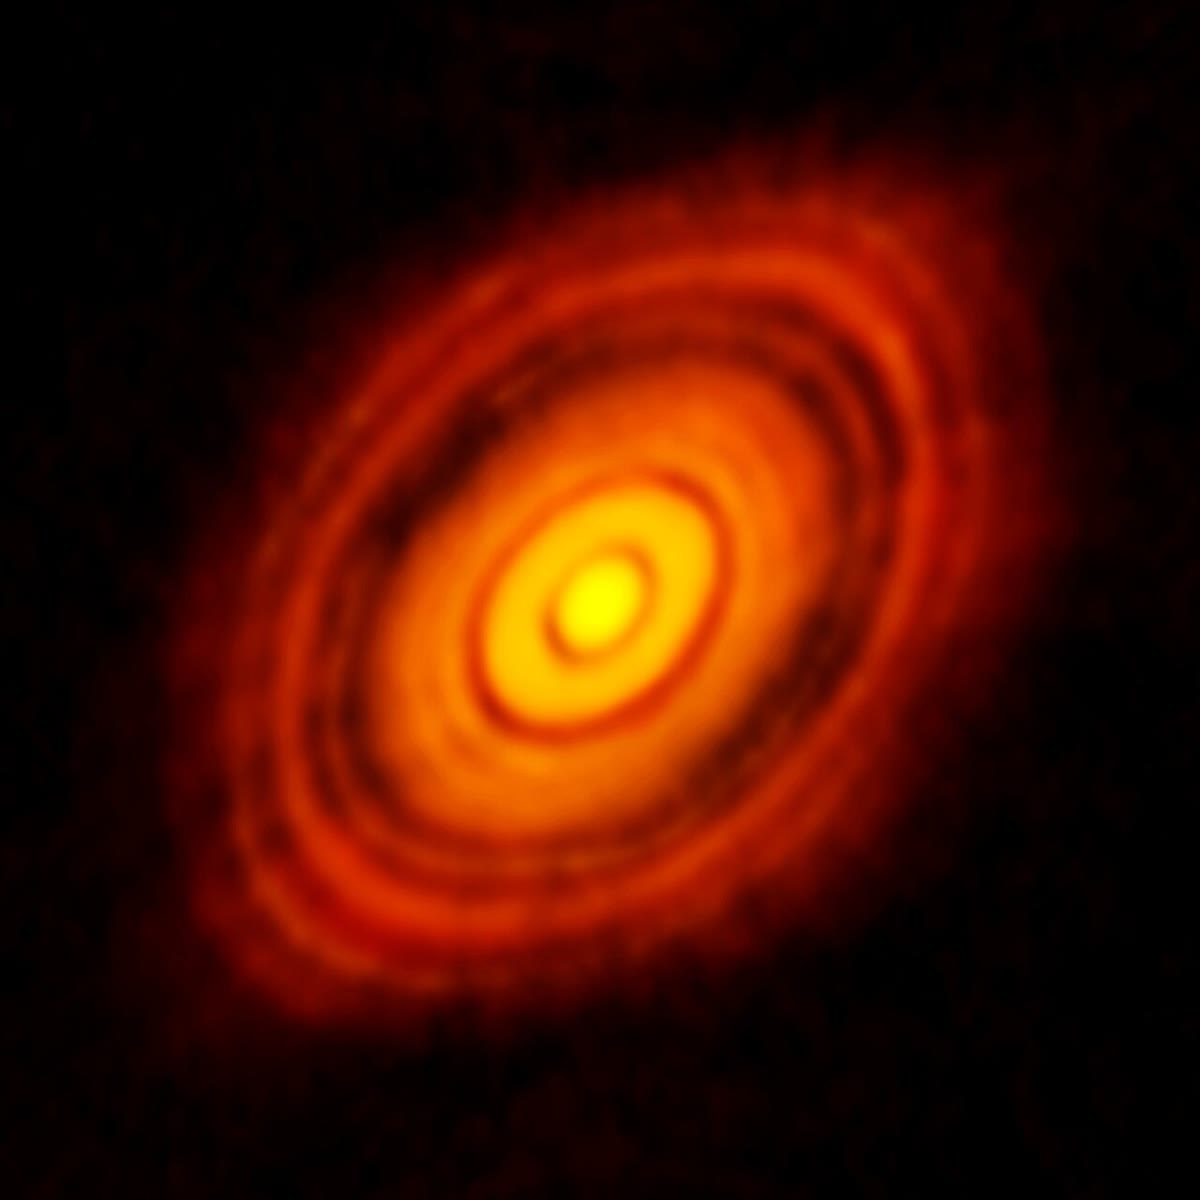
\includegraphics[width=\linewidth]{images/book4/b2-hl-tau-alma.jpg}
\end{minipage}\hfill
\begin{minipage}[c]{0.52\linewidth}
{\small 年轻恒星 HL 金牛座的盘，距离 \qty{140}{pc}，位于金牛座，
由 ALMA 干涉仪在约一毫米波长下成像，此波长处冷
尘埃发光。该盘半径约 \qty{120}{au}，以
\ang{47} 倾角观测，呈现出宽约几个天文单位的明暗相间的环；
该系统至多一两百万年，这些环被解读为
行星清出其轨道的最早迹象。ALMA（ESO/NAOJ/NRAO），CC BY 4.0。}
\end{minipage}
% ledger: alma:hltau
\end{omfigure}

圆盘受恒星加热。距离为 $r$ 处的尘粒沿其截面吸收星光，
并从整个表面辐射。

\begin{proposition}[星光照射下尘粒的温度]
\label{prop:b2:ism-star-formation:grain}
一颗行为如黑体的小尘粒，位于距恒星 $r$ 处（恒星光度为 $L$），
且仅一侧受阳光照射，其平衡温度为
\[
  T = \left(\frac{L}{16\pi\sigma r^2}\right)^{1/4},
\]
其温度按 $r^{-1/2}$ 的规律下降。
\end{proposition}

\begin{proof}
半径为 $a$ 的球形尘粒截获的功率为 $\pi a^2\,L/(4\pi r^2)$，
在温度 $T$ 下，其表面辐射 $4\pi a^2\sigma T^4$。
平衡时两者相等：$T^4 = L/(16\pi\sigma r^2)$；$a$ 相消。
\end{proof}

在与太阳类似的恒星的 \qty{1}{au} 处，尘粒温度为 \qty{278}{K}；在
木星轨道所在的 \qty{5.2}{au} 处，温度为 \qty{122}{K}。水冰
凝结于尘粒温度低于约 \qty{180}{K} 的地方（凝聚温度见
\cref{ch:b2:planet-formation-meteorites}），即在约
\qty{2.4}{au} 之外：这便是分界线的最初迹象，即雪线，它将岩质行星与冰质行星分隔开来。
真实的圆盘是不透明的，其中平面受到遮挡，不直接接受星光；
该命题给出了正确的数量级，并且
对恒星所照射的表层给出了正确的斜率。
% ledger: lodders:tc-table

圆盘并不能长久存在。红外超量，即高于恒星自身所能发出的辐射之上的温暖尘埃所发出的辉光，
可以揭示一颗恒星是否仍拥有圆盘。统计
不同年龄星团中具有这种超量的恒星数目，便得到保留圆盘的恒星比例
随时间变化的规律（见下图）：大多数恒星出生时都有圆盘，
到约 300 万年时半数已失去圆盘，超过 600 万年时
几乎没有恒星仍保留圆盘。气态巨行星必须从圆盘中汲取气体，
因此它们必须在这短短几百万年内形成。
% ledger: haisch:disc-fractions, haisch:disc-lifetime

\begin{omfigure}
\begin{tikzpicture}
\begin{axis}[omrecord, width=0.8\linewidth, height=5.6cm, xmin=0, xmax=8.5, ymin=0, ymax=1.05,
  xlabel={星团年龄（Ma）}, ylabel={具有圆盘的恒星比例},
  tick label style={font=\scriptsize}, label style={font=\small}, clip=false]
\addplot[thick, black!55, densely dashed] table[x=age, y=frac] {figdata/out/bachelor-2-jeans-discfit.dat};
\addplot[only marks, mark=*, mark size=1.8pt, blue!70!black,
  error bars/.cd, y dir=both, y explicit]
  table[x=age, y=frac, y error=err, restrict x to domain=0:10] {figdata/out/bachelor-2-jeans-discs.dat};
\node[font=\scriptsize, anchor=north west] at (axis cs:0.05,0.74) {NGC 2024};
\node[font=\scriptsize, anchor=south west] at (axis cs:1.55,0.86) {猎户四边形星团};
\node[font=\scriptsize, anchor=south west] at (axis cs:2.35,0.71) {IC 348};
\node[font=\scriptsize, anchor=south west] at (axis cs:3.3,0.56) {NGC 2264};
\node[font=\scriptsize, anchor=south west] at (axis cs:5.1,0.15) {NGC 2362};
\node[font=\scriptsize, anchor=north east] at (axis cs:8.4,0.98) {(NGC 1960, \qty{30}{Ma}: $0.03$)};
\end{axis}
\end{tikzpicture}

\par\smallskip{\small 年轻星团中呈现圆盘红外超量的恒星比例，
随星团年龄（及其误差）变化，数据取自 Haisch、Lada
和 Lada（2001）。虚线为对五个最年轻星团所作的
最小二乘直线：它在 \qty{3.0}{Ma} 处达到 $0.5$，在 \qty{6.1}{Ma} 处为零
（见\cref{exo:b2:ism-star-formation:12}）。}
\end{omfigure}

\begin{inthelab}[用射电波透视尘埃]
\begin{minipage}[t]{0.55\linewidth}\vspace{0pt}
冷气体和尘埃对光学望远镜不可见，但它们在毫米波段发光，
而该波段的大气仅在高海拔干燥台址之上才透明。一座
房屋大小的射电天线在这些波长上分辨率很低，因此天文学家
将许多天线组合起来：在干涉仪中，每一对天线
由一条基线隔开，测量天空亮度分布的一个分量，
再由计算机从约三十台天线构成的数百对组合中合成图像。分辨率
等同于一台口径与最长基线相同的单一望远镜：天线分布在
\qty{15}{km} 的范围内时，HL 金牛座圆盘在
\qty{140}{pc} 处被以几个天文单位的细节成像。操作人员在不同构型之间用转运装置移动天线，
相关器则实时合成它们的信号。
\end{minipage}\hfill
\begin{minipage}[t]{0.42\linewidth}\vspace{0pt}
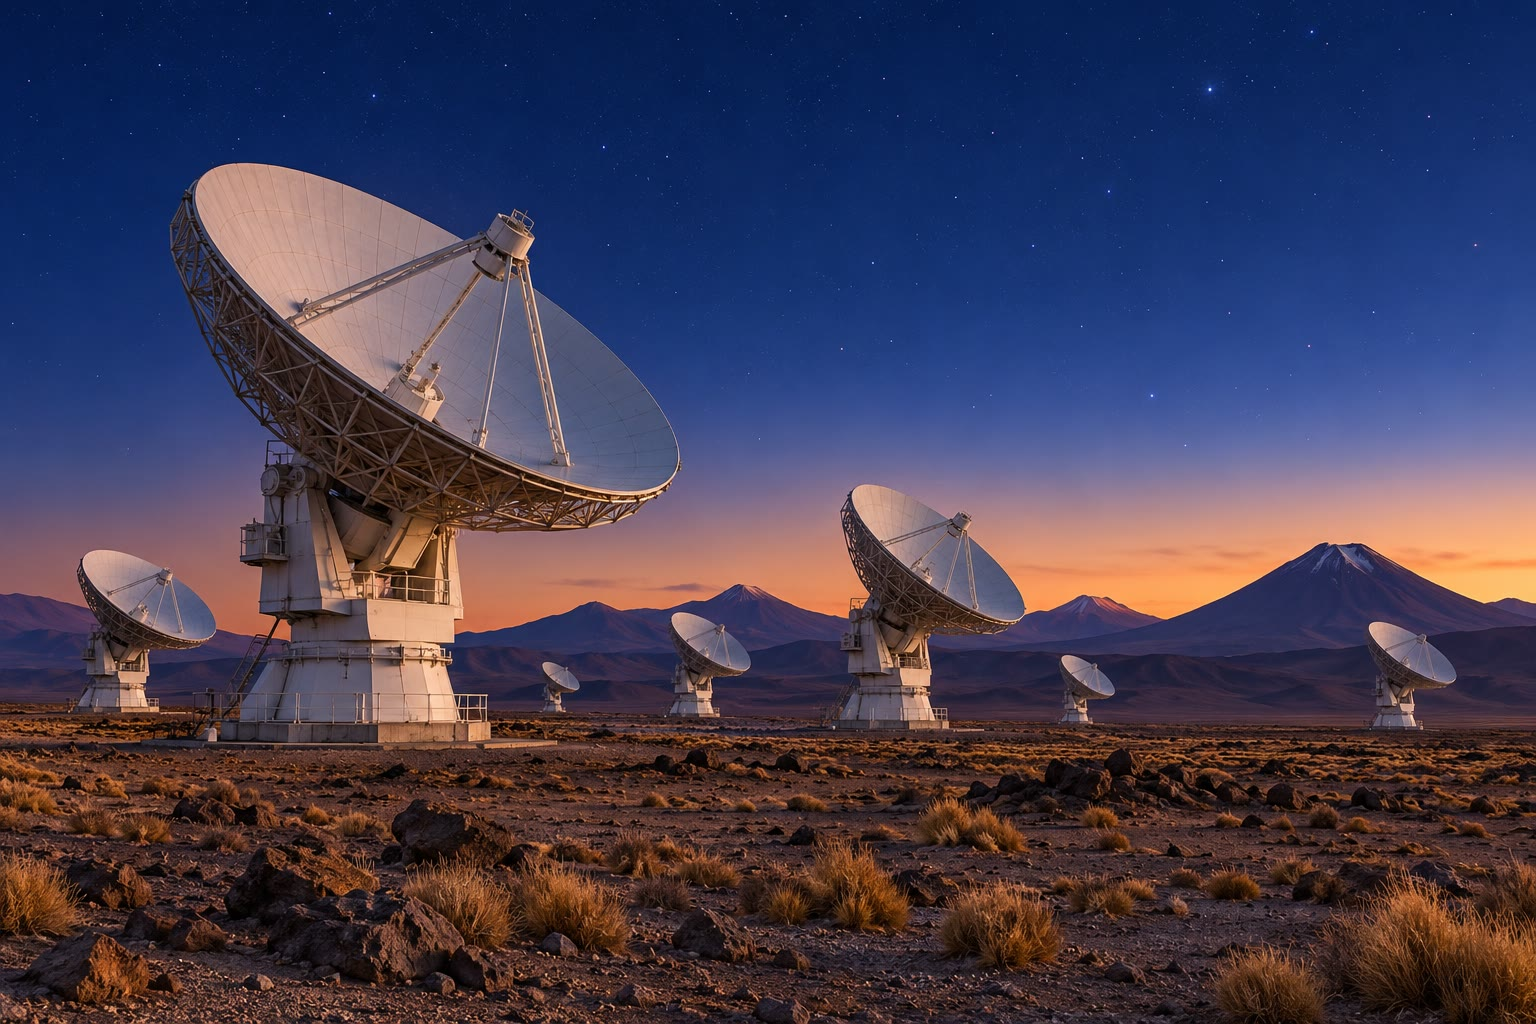
\includegraphics[width=\linewidth]{images/book4/ai/b2-radio-array.jpg}

{\scriptsize 黄昏时分位于高海拔沙漠高原上的一组射电天线
（AI 生成插图）。}
\end{minipage}
% ledger: alma:hltau, alma:baselines
\end{inthelab}

\section{练习}

\begin{exercise}[$\star$]\label{exo:b2:ism-star-formation:1}
太阳附近\omterm{def:b2:ism-star-formation:ism}{星际介质}的平均密度为 \qty{2.7e-24}{g.cm^{-3}}。取
氢原子质量为 \qty{1.67e-24}{g}，求每立方厘米内的
氢原子数。将其与空气中每立方厘米的
分子数进行比较（空气处于 \qty{101325}{Pa}、\qty{288}{K}，$n = P/k_{\mathrm B}T$）。
% ledger: ferriere:mean-density, const:kB
\end{exercise}

\begin{exercise}[$\star$]\label{exo:b2:ism-star-formation:2}
取 \qty{10}{K} 时\omterm{def:b2:ism-star-formation:jeans}{金斯质量} $M_J = 5.46$ 个太阳质量（对应 $10^4$ 个粒子每立方厘米），
并利用 $M_J$ 随密度的标度关系，求 \qty{10}{K}、$10^2$ 个粒子
每立方厘米时的\omterm{def:b2:ism-star-formation:jeans}{金斯质量}。金牛座\omterm{def:b2:ism-star-formation:molecular-cloud}{分子云}
质量为 \num{24000} 个太阳质量，它包含多少个\omterm{def:b2:ism-star-formation:jeans}{金斯质量}？
% ledger: goldsmith:taurus-mass
\end{exercise}

\begin{exercise}[$\star$]\label{exo:b2:ism-star-formation:3}
计算分子气体的等温声速 $c_s = (k_{\mathrm B}T/\mu m_u)^{1/2}$，
（$\mu = 2.33$，$m_u = \qty{1.661e-27}{kg}$），求其在 \qty{10}{K} 和 \qty{100}{K} 时的值。
在 \qty{10}{K} 时，声波穿过半径为
\qty{0.1}{pc} 的\omterm{def:b2:ism-star-formation:molecular-cloud}{致密云核}需要多长时间，以百万年计？
% ledger: kauffmann:mu, nist:u, iau:parsec
\end{exercise}

\begin{exercise}[$\star$]\label{exo:b2:ism-star-formation:4}
计算数密度为每立方厘米 $10^5$ 个粒子的\omterm{def:b2:ism-star-formation:molecular-cloud}{致密云核}
及数密度为 $10^2$（$\mu = 2.33$）的暗云的\omterm{def:b2:ism-star-formation:free-fall}{自由落体时标}。哪一个坍缩
更快，快多少倍？
\end{exercise}

\begin{exercise}[$\star\star$]\label{exo:b2:ism-star-formation:5}
证明 $M_J$ 可以写成 $M_J = 5^{3/2}\,(3/4\pi)^{1/2}\,c_s^3\,G^{-3/2}\rho^{-1/2}$。
温度保持不变时，云核的密度需升至原来的多少倍，
才能使其\omterm{def:b2:ism-star-formation:jeans}{金斯质量}减半？密度保持不变时，
若云核从 \qty{10}{K} 升温到 \qty{20}{K}，\omterm{def:b2:ism-star-formation:jeans}{金斯质量}变为原来的多少倍？
\end{exercise}

\begin{exercise}[$\star\star$]\label{exo:b2:ism-star-formation:6}
一颗年轻恒星的质量与太阳相同，其半径和光度均为太阳的两倍，
（$M_\odot = \qty{1.989e30}{kg}$，$R_\odot = \qty{6.96e8}{m}$，
$L_\odot = \qty{3.83e26}{W}$）。计算其\omterm{def:b2:ism-star-formation:kh-time}{开尔文–亥姆霍兹时标}，以百万年计，
并与盘的寿命作比较。
% ledger: sun:mass, sun:R, sun:L
\end{exercise}

\begin{exercise}[$\star\star$]\label{exo:b2:ism-star-formation:7}
计算温度为 \qty{10}{K} 的云核中\omterm{def:b2:ism-star-formation:protostar}{原恒星}的吸积率 $c_s^3/G$，以太阳质量每年计，
以及积累一个太阳质量所需的时间。对
温度为 \qty{20}{K} 的云核，同样回答上述问题。
\end{exercise}

\begin{exercise}[$\star\star$]\label{exo:b2:ism-star-formation:8}
结合\cref{prop:b2:ism-star-formation:grain}及 $L_\odot = \qty{3.83e26}{W}$，求尘埃颗粒
达到 \qty{1300}{K} 时距太阳的距离（以天文单位计）。该温度接近
常见硅酸盐凝结的温度（见\cref{ch:b2:planet-formation-meteorites}），
以及尘埃颗粒在木星距离
\qty{5.2}{au} 处的温度。
% ledger: sun:L, const:sigma, const:au
\end{exercise}

\begin{exercise}[$\star\star$]\label{exo:b2:ism-star-formation:9}
HL Tauri 盘中的气体绕一颗质量约为 \num{1.3} 个
太阳质量的恒星旋转。求 \qty{100}{au} 处的开普勒速度和轨道周期。
若该系统的年龄为一百万年，
则自恒星形成以来，\qty{100}{au} 处的气体已转过多少圈？
% ledger: alma:hltau
\end{exercise}

\begin{exercise}[$\star\star\star$]\label{exo:b2:ism-star-formation:10}
求半径为 $R$ 的球体的引力能，其中密度
按 $\rho(r) = \rho_0 R/r$ 下降，并将其与质量和半径相同的
均匀球体的引力能作比较。质量向中心集中后，
云团是更容易还是更难由其热能支撑？
\end{exercise}

\begin{exercise}[$\star\star\star$]\label{exo:b2:ism-star-formation:11}
半径为 \qty{0.1}{pc} 的云核以角速度
$\Omega = \qty{1e-14}{rad.s^{-1}}$ 做刚体转动。求其转动周期，以及赤道处气体的
比角动量 $j = \Omega R^2$，并求该气体绕一颗太阳质量恒星的离心
半径（以天文单位计）。
为何云核内部的气体落在离恒星更近的位置？
\end{exercise}

\begin{exercise}[$\star\star\star$]\label{exo:b2:ism-star-formation:12}
上一节图中五个最年轻星团的含盘比例分别为
$0.85$、$0.80$、$0.65$、$0.52$ 和 $0.12$，对应年龄分别为 0.3、1.5、2.3、3.2 和
\qty{5.0}{Ma}。用手工拟合最小二乘直线 $f = a - bt$（先求均值，
再计算 $\sum(t - \bar t)(f - \bar f)$ 与
$\sum(t - \bar t)^2$）。该直线在何年龄降到一半，又在何年龄降到零？为何
超过该年龄后直线是一个较差的模型？
% ledger: haisch:disc-fractions
\end{exercise}

\section{问题：Aldra 暗云中的一个云核}

\begin{problem}[{周末问题——由一张尘埃图读出致密云核的质量与稳定性、
其原恒星的诞生以及盘的大小}]
\label{pb:b2:ism-star-formation:1}
% values: calc/ch01.py
% ledger: kauffmann:mu, nist:u, iau:parsec, const:G, const:kB, sun:mass, sun:R, sun:L, const:au, const:sigma, bt07:cores, alma:hltau
Aldra 暗云为虚构的暗云。其尘埃的毫米波图
显示出一个半径为 \qty{0.08}{pc} 的圆形云核，其平均柱密度为
$N(\ce{H2}) = \num{1.5e22}$ 个氢分子每平方厘米。一条
氨谱线给出气体温度 \qty{10}{K}，并给出
跨越云核的速度梯度为每秒差距 \qty{0.4}{km.s^{-1}}，
按刚体转动解读。采用 $G = \qty{6.674e-11}{m^3.kg^{-1}.s^{-2}}$，
$k_{\mathrm B} = \qty{1.381e-23}{J.K^{-1}}$，$m_u = \qty{1.661e-27}{kg}$，
\qty{1}{pc} $= \qty{3.086e16}{m}$，\qty{1}{au} $= \qty{1.496e11}{m}$，一年为
\qty{3.156e7}{s}，$M_\odot = \qty{1.989e30}{kg}$，$R_\odot = \qty{6.96e8}{m}$，
$L_\odot = \qty{3.83e26}{W}$，$\sigma = \qty{5.67e-8}{W.m^{-2}.K^{-4}}$；
每个氢分子的质量（计入氦）为 $2.8\,m_u$，平均每个粒子的质量为
$2.33\,m_u$。

\medskip
\noindent\textbf{第一部分——质量与密度。}
\begin{enumerate}
  \item 将云核的半径换算为米。
  \item 计算柱内每平方米的质量 $2.8\,m_u N$。
  \item 由此求云核的质量，分别以千克和太阳质量表示。
  \item 计算其体积和平均密度。
  \item 计算每立方厘米的粒子数。
  \item 按第二节表中的定义，这是一个\omterm{def:b2:ism-star-formation:molecular-cloud}{致密云核}吗？
\end{enumerate}

\noindent\textbf{第二部分——稳定性。}
\begin{enumerate}[resume]
  \item 计算云核气体的\omterm{def:b2:ism-star-formation:jeans}{金斯质量}，以太阳质量为单位。
  \item 云核包含多少个\omterm{def:b2:ism-star-formation:jeans}{金斯质量}？它是否稳定？
  \item 计算\omterm{def:b2:ism-star-formation:jeans}{金斯长度}，并将其与云核的半径作比较。
  \item 若气体温度为 \qty{20}{K}，\omterm{def:b2:ism-star-formation:jeans}{金斯质量}将为多少？云核
        仍会坍缩吗？
  \item 计算云核的\omterm{def:b2:ism-star-formation:free-fall}{自由落体时标}，以千年计。
  \item 将其与声波穿过云核所需的时间作比较。哪一个
        过程更快，这说明什么？
\end{enumerate}

\noindent\textbf{第三部分——\omterm{def:b2:ism-star-formation:protostar}{原恒星}。}
\begin{enumerate}[resume]
  \item 计算云核中的声速。
  \item 计算吸积率 $c_s^3/G$，以太阳质量每年为单位。
  \item 计算以此速率积聚一个太阳质量所需的时间。
  \item 若云核的三分之一最终转化为恒星，则它
        能形成多少颗一个太阳质量的恒星？
  \item 包层消散后，该恒星的质量为一个太阳质量，半径为
        三个太阳半径，光度为四个太阳光度。计算其\omterm{def:b2:ism-star-formation:kh-time}{开尔文–亥姆霍兹时标}。
  \item 该时标比吸积时间长还是短？此时它是
        哪一类恒星？
\end{enumerate}

\noindent\textbf{第四部分——圆盘。}
\begin{enumerate}[resume]
  \item 将速度梯度换算为角速度 $\Omega$，
        以 \unit{rad.s^{-1}} 为单位。
  \item 计算位于云核赤道处气体的比角动量
        $j = \Omega R^2$。
  \item 计算其围绕一个太阳质量恒星的离心半径，
        以天文单位表示。
  \item 计算尘粒在 \qty{1}{au} 和 \qty{30}{au} 处的温度，
        其热源为光度等于一个太阳光度的恒星。
  \item 若水冰在低于 \qty{180}{K} 时仍能存留，
        求该圆盘雪线的位置。
  \item 求出组装第 15 题中恒星所需的时间，
        即本题的关键数值，以千年计，
        并将其与第 11 题中的\omterm{def:b2:ism-star-formation:free-fall}{自由落体时标}作比较。
\end{enumerate}
\end{problem}
